Objectifs du cours

Donner les outils permettant de déterminer les rapports de transmission
des transmetteurs usuels.

Savoirs

Je connais~:

\begin{center}\begin{tabular}[]{@{}
  >{\raggedright\arraybackslash}p{0.9045\linewidth}
  >{\raggedright\arraybackslash}p{0.0955\linewidth}@{}}

\begin{minipage}[b]{\linewidth}\raggedright
\begin{itemize}
\item
  la démarche permettant de déterminer une loi entrée-sortie~;
\end{itemize}
\end{minipage} & \begin{minipage}[b]{\linewidth}\raggedright
$\bigcirc$
\end{minipage} \\




\begin{minipage}[t]{\linewidth}\raggedright
\begin{itemize}
\item
  la notion de modèle géométrique direct et inverse;
\end{itemize}
\end{minipage} & $\bigcirc$ \\
\begin{minipage}[t]{\linewidth}\raggedright
\begin{itemize}
\item
  la notion de coordonnées articulaires et opérationnelles~;
\end{itemize}
\end{minipage} & $\bigcirc$ \\
\begin{minipage}[t]{\linewidth}\raggedright
\begin{itemize}
\item
  les symboles permettant de représenter les transmetteurs usuels~;
\end{itemize}
\end{minipage} & $\bigcirc$ \\
\begin{minipage}[t]{\linewidth}\raggedright
\begin{itemize}
\item
  les différentes méthodes et formules pour déterminer le rapport de
  réduction d'un engrenage simple, d'un train d'engrenage simple, d'un
  train d'engrenage épicycloïdal et d'un roue et vis sans fin.
\end{itemize}
\end{minipage} & $\bigcirc$ \\
\end{tabular}\end{center}

Savoir-faire

Je sais~:

\begin{center}\begin{tabular}[]{@{}
  >{\raggedright\arraybackslash}p{0.9045\linewidth}
  >{\raggedright\arraybackslash}p{0.0955\linewidth}@{}}

\begin{minipage}[b]{\linewidth}\raggedright
\begin{itemize}
\item
  déterminer le rapport de réduction d'un engrenage simple~;
\end{itemize}
\end{minipage} & \begin{minipage}[b]{\linewidth}\raggedright
$\bigcirc$
\end{minipage} \\




\begin{minipage}[t]{\linewidth}\raggedright
\begin{itemize}
\item
  déterminer le rapport de réduction d'un train d'engrenage simple~;
\end{itemize}
\end{minipage} & $\bigcirc$ \\
\begin{minipage}[t]{\linewidth}\raggedright
\begin{itemize}
\item
  déterminer le rapport de réduction d'un train d'engrenage
  épicycloïdal~;
\end{itemize}
\end{minipage} & $\bigcirc$ \\
\begin{minipage}[t]{\linewidth}\raggedright
\begin{itemize}
\item
  déterminer le rapport de réduction d'un roue et vis sans fin~;
\end{itemize}
\end{minipage} & $\bigcirc$ \\
\begin{minipage}[t]{\linewidth}\raggedright
\begin{itemize}
\item
  déterminer le rapport de réduction d'un pignon-crémaillère, vis-écrou,
  d'un poulie-courroie et pignons-chaine.
\end{itemize}
\end{minipage} & $\bigcirc$ \\
\end{tabular}\end{center}

\subsection{MISE EN SITUATION}\label{mise-en-situation}

\subsubsection{Cas n°1~: Objectif d'appareil
photo}\label{cas-n1-objectif-dappareil-photo}


\includegraphics[width=\linewidth,height=.72\textheight,keepaspectratio]{images/image5.png}L'autofocus
(AF) est le terme anglais pour désigner la mise au point automatique.
C'est une fonction qui permet la mise au point automatique de certains
systèmes optiques comme les appareils photo, leur permettant de régler
la netteté du sujet. Cette mise au point est réalisée grâce à
l'association d'un boitier et d'un objectif photographiques.

Le principe consiste à déplacer une lentille afin que les rayons de
l'image à photographier convergent sur le capteur. Si ce n'est pas le
cas, l'image sera floue. Sur la figure 2, la lentille est bien
positionnée uniquement sur le schéma du milieu : les rayons convergent
parfaitement sur le capteur.


\includegraphics[width=\linewidth,height=.72\textheight,keepaspectratio]{images/image6.png}

Le mouvement de la lentille est donné par l'architecture représentée
ci-après.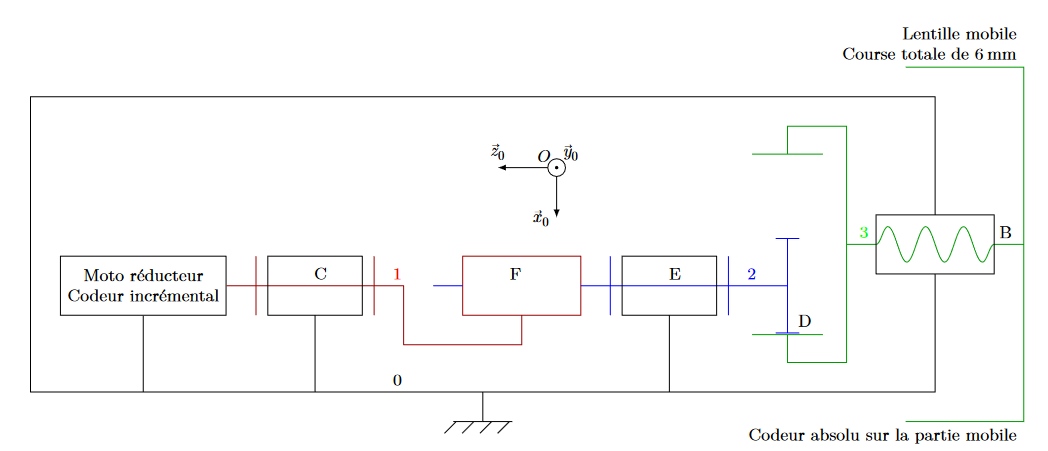
\includegraphics[width=\linewidth,height=.72\textheight,keepaspectratio]{images/image7.png}


\includegraphics[width=\linewidth,height=.72\textheight,keepaspectratio]{images/image8.png}


\includegraphics[width=\linewidth,height=.72\textheight,keepaspectratio]{images/image9.png}

Pour vérifier la résolution annoncée par le constructeur, il faut
trouver le rapport de transmission entre le moteur et la lentille.

\subsection{GRANDEURS D'ENTREE ET DE SORTIE, LOI ENTREE-SORTIE
CINEMATIQUE}\label{grandeurs-dentree-et-de-sortie-loi-entree-sortie-cinematique}

Pour tous les systèmes, le mouvement d\textquotesingle entrée est
généralement continu, alors que le mouvement de sortie peut être,
continu, alterné ou intermittent. Lorsque l'entrée et la sortie peuvent
être permutées, on dit que le système est \textbf{réversible} (dans le
cas contraire, il est \textbf{irréversible}).

On a vu dans le cours précédent des \textbf{démarches} permettant
d'établir des \textbf{relations} mathématiques entre les
\textbf{paramètres de mouvement} et les \textbf{caractéristiques
géométriques} d'un mécanisme afin d'assurer un \textbf{comportement
cinématique de l'effecteur d'une chaîne de puissance imposé} par un
cahier des charges.

Pour pouvoir remonter jusqu'aux \textbf{lois de commande} des
préactionneurs délivrant la puissance aux actionneurs à l'origine de ces
mouvements imposés, il faut très souvent tenir compte de la \textbf{loi
entrée-sortie cinématique des transmetteurs} présent dans la chaîne de
puissance.


\includegraphics[width=\linewidth,height=.72\textheight,keepaspectratio]{images/image10.png}

L'objectif de ce cours de \textbf{modéliser le comportement cinématique
des transmetteurs usuels}.

La description de la chaîne de puissance permet, pour chaque
transmetteur, de définir des grandeurs d'entrée et des grandeurs de
sortie.

Et aussi : pignon-chaîne, roue et vis sans fin\ldots{} Et aussi : came,
bielle-manivelle\ldots{}

Une \textbf{loi entrée-sortie} d'un transmetteur est une
\textbf{relation mathématique}, imposée par la \textbf{structure} du
transmetteur, entre une ou des \textbf{grandeurs d'entrée} et une ou des
\textbf{grandeurs de sortie}.

Une loi entrée-sortie cinématique caractérise le comportement
cinématique du composant de la chaîne de puissance, elle en est le
modèle cinématique.

Exemples~: \(\omega_{s} = f\left( \omega_{e} \right)\) ou
\(v_{s} = f(\omega_{e})\)

La loi entrée sortie cinématique est donnée par le \textbf{rapport de
transmission} \(\mathbf{r\ }\)qui est le rapport entre la vitesse
angulaire de sortie \(\omega_{s}\) et la vitesse angulaire d'entrée
\(\omega_{e}\)\emph{~}:
\(k = \frac{\omega_{s}}{\omega_{e}} = \frac{\dot{\theta_{s}}}{\dot{\theta_{e}}}\)
ou
\(k = \frac{v_{s}}{\omega_{e}} = \frac{\dot{{\lambda\ }_{s}}}{\dot{\theta_{e}}}\)
pour les deux cas précédents.

\subsection{Eléments de transmission de
puissance}\label{eluxe9ments-de-transmission-de-puissance}

\subsubsection{Classification des éléments de transmission de
puissance}\label{classification-des-uxe9luxe9ments-de-transmission-de-puissance}

Il existe deux types de mouvements élémentaires : la translation et la
rotation. Tous les mouvements ne sont qu'association ou combinaison des
deux.

Une transformation de mouvement se caractérise par une différence entre
le mouvement moteur et le mouvement récepteur. Cette différence peut
être simple ou multiple parmi les suivantes~: nature, direction, sens,
vitesse du mouvement.

\emph{\hfill\break
}

\subsection{TRANSMETTEURS LINEAIRES SANS TRANSFORMATION DE MOUVEMENT~:
LES REDUCTEURS ET LES
MULTIPLICATEURS}\label{transmetteurs-lineaires-sans-transformation-de-mouvement-les-reducteurs-et-les-multiplicateurs}

\subsubsection{Loi entrée-sortie cinématique : rapport de
transmission}\label{loi-entruxe9e-sortie-cinuxe9matique-rapport-de-transmission}

\begin{quote}

\includegraphics[width=\linewidth,height=.72\textheight,keepaspectratio]{images/image15.png}
\end{quote}

On nomme souvent les transmetteurs linéaires \textbf{réducteur ou
multiplicateur de vitesse}, mais ils agissent aussi sur le couple
transmis en faisant intervenir le rendement.

La loi entrée sortie cinématique est donnée par le \textbf{rapport de
transmission} \(\mathbf{r\ }\)qui est le rapport entre la vitesse
angulaire de sortie \(\omega_{s}\) et la vitesse angulaire d'entrée
\(\omega_{e}\)\emph{~}:

\(r = \frac{\omega_{s}}{\omega_{e}} = \frac{\dot{\theta_{s}}}{\dot{\theta_{e}}}\)

Parfois on parle d'un rapport de réduction de 150. Il faut traduire que
le rapport de réduction est de 1/150

'\,'

Selon la valeur de ce rapport (\textless1 ou \textgreater1), on parle de
\textbf{multiplicateur} ou de \textbf{réducteur} de vitesse.

Dans le cas d'un réducteur de vitesse, il y a multiplication du couple
(et inversement pour un multiplicateur). Néanmoins, le rapport des
couples fait intervenir le rendement \(\eta\) .

\[\eta = \frac{P_{s}}{P_{e}} = \frac{C_{s}\omega_{s}}{C_{e}\omega_{e}} = \frac{C_{s}}{C_{e}}r\]

Rappel~: \(\Omega_{m} = \ \frac{2\pi N_{m}}{60}\) pour passer de
tr.min\textsuperscript{-1} à rad.s\textsuperscript{-1}

\subsubsection{\texorpdfstring{\textbf{Transmetteur par adhérence~:
roues de
friction}}{Transmetteur par adhérence~: roues de friction}}\label{transmetteur-par-adhuxe9rence-roues-de-friction}

\textbf{Principe}

Deux roues cylindriques sont en contact. L'adhérence permet d'assurer le
roulement sans glissement au point \emph{I} de contact des roues, et
donc de transmettre le mouvement de la roue 1 dite \emph{« menante »} à
la roue 2 dite \emph{« menée »}.


\includegraphics[width=\linewidth,height=.72\textheight,keepaspectratio]{images/image20.png}

Pour assurer un roulement sans glissement il faut utiliser :

\begin{itemize}
\item
  un couple de matériaux avec un fort coefficient d'adhérence
\item
  un effort presseur entre les deux roues (via un ressort par exemple)
\end{itemize}

\textbf{Applications}

Transmissions de faible puissance comme dynamo de vélo,
home-trainer\ldots{}

\textbf{Rapport de transmission}

En utilisant le roulement sans glissement en A (s'il y a adhérence,
c'est-à-dire si cela ne patine pas au niveau du point de contact entre
les deux roues) entre les roues \ul{1} et \ul{2}
(\(\overrightarrow{\text{V}_{\text{A, 1/2}}} = \overrightarrow{0})\), on
démontre que le rapport de réduction est~:
\(\frac{\text{\ensuremath{\omega}}_{\text{2/0}}}{\text{\ensuremath{\omega}}_{\text{1/0}}}\text{=-}\frac{\text{d}_{\text{1}}}{\text{d}_{\text{2}}}\)

\textbf{Limites du dispositif}

La puissance transmise par ce dispositif est très limitée. En effet pour
augmenter la puissance transmissible il faudrait :

\begin{itemize}
\item
  Augmenter le facteur de frottement entre « 1 » et « 2 »~: il dépend de
  la nature des matériaux de « 1 » et de « 2 » et est maximal lorsque «
  1 » est en caoutchouc.
\item
  Augmenter l'effort presseur.
\end{itemize}

Cette solution est donc possible pour les faibles puissances et reste
limitée car elle nécessite des pressions de contact importantes pour
assurer le roulement sans glissement. Exemples~d'utilisation~:
transmission de puissance d'un ancien vélo SOLEX, entrainement du
plateau d'un ancien Tourne disque, baladeur\ldots{} Pour pallier cette
difficulté, on réalise des transmissions par obstacle.

\subsubsection{Transmission par obstacle~: engrenage
simple}\label{transmission-par-obstacle-engrenage-simple}

Un \textbf{engrenage} est constitué de \textbf{deux \emph{roues
dentées}} qui engrènent l'une avec l'autre. La géométrie de la denture
permet d'obtenir la même cinématique que celle imposée par deux roues de
friction. La petite roue dentée est parfois appelée « \textbf{pignon} »
et la grande « \textbf{roue} » (ou « \textbf{couronne} » dans le cas
d'un engrenage intérieur).


\includegraphics[width=\linewidth,height=.72\textheight,keepaspectratio]{images/image21.png}

\textbf{Diamètre primitif}


\includegraphics[width=\linewidth,height=.72\textheight,keepaspectratio]{images/image22.png}L'engrènement
de dentures assure le roulement sans glissement en I des cercles fictifs
de diamètres D\textsubscript{1} et D\textsubscript{2}. Ces cercles sont
appelés \textbf{cercles primitifs}. Ils correspondent aux diamètres des
roues de friction qui assureraient le même rapport de transmission.

\textbf{Pas primitif}

Pour garantir cet engrènement, les \textbf{pas primitifs} respectifs des
dentures du pignon et de la roue, qui correspondent aux longueurs des
arcs des cercles primitifs compris entre deux profils de dents
consécutifs (le pas primitif est la distance, sur le cercle primitif,
entre deux dents), doivent être égaux~:
\(pas = \frac{2\pi.R_{1}}{Z_{1}} = \frac{2\pi.R_{2}}{Z_{2}} = \pi m\)

On a donc : \(\text{p=}\frac{\text{\ensuremath{\pi}d}}{\text{Z}} = \pi m\) (Z est le
nombre de dents)

\textbf{Deux roues engrenant doivent avoir le même pas primitif} p,
\(\frac{\text{\ensuremath{\pi}}d_{1}}{Z_{1}} = \frac{\text{\ensuremath{\pi}}d_{2}}{Z_{2}}\)

\textbf{Donc deux roues qui n'ont pas le même module ne peuvent pas
engrener car leur pas est différent.}

\textbf{Module}

Le module (symbolisé m) caractérise l'aptitude à l'engrènement des
diverses roues entre elle. Pour que deux roues puissent engrener, il
faut impérativement qu'elles aient le \emph{même module m}. Le module
est une dimension normalisée qui caractérise la forme des dents.


\includegraphics[width=\linewidth,height=.72\textheight,keepaspectratio]{images/image23.png}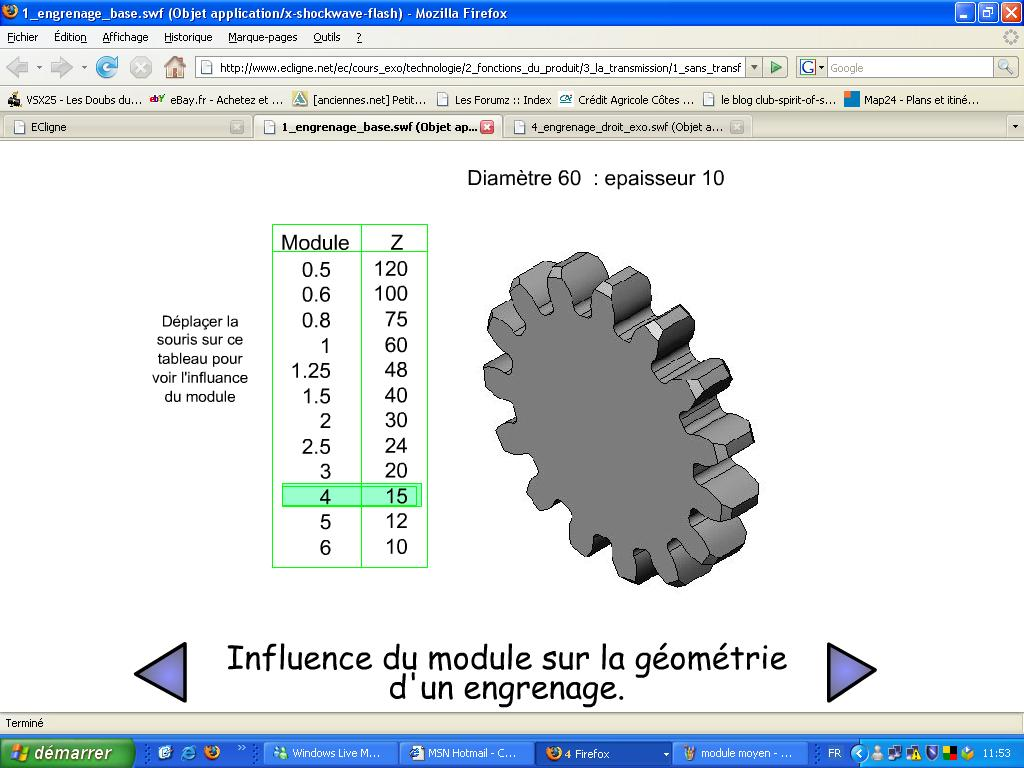
\includegraphics[width=\linewidth,height=.72\textheight,keepaspectratio]{images/image24.jpeg}On
montre que~: \(d = m \times Z\)

Avec :

d : diamètre primitif en mm

m : module en mm

Z : nombre de dents

\textbf{Angle de pression \ensuremath{\alpha}}


\includegraphics[width=\linewidth,height=.72\textheight,keepaspectratio]{images/image25.png}Autre
caractéristique importante d'un engrenage, il définit l'inclinaison de
la ligne de pression \ensuremath{\Delta}. La valeur la plus utilisée est \ensuremath{\alpha}=20 °

Les efforts dans les dentures apparaissent au contact des dents sous
trois composantes perpendiculaires les unes aux autres.

\begin{itemize}
\item
  L'effort axial « Fa » : parallèle à l'axe de l'arbre, il devra être
  transmis au carter par l'intermédiaire d'un roulement à rouleaux
  conique le plus souvent. Le guidage en rotation devra encaisser.
\item
  L'effort tangentiel « Ft » : Tangent au cône primitif et
  perpendiculaire à l'axe, « FT » est le seul effort qui participe à la
  transmission de puissance.
\item
  L'effort radial « Fr » : Perpendiculaire aux deux autres, cet effort
  peut engendrer une flexion de l'arbre si ce dernier est sous
  dimensionné.
\end{itemize}

\textbf{Caractéristiques des roues dentées}

\begin{center}\begin{tabular}[]{@{}
  >{\raggedright\arraybackslash}p{0.1896\linewidth}
  >{\raggedright\arraybackslash}p{0.8104\linewidth}@{}}

\begin{minipage}[b]{\linewidth}\raggedright
\textbf{Diamètre primitif}
\end{minipage} & \begin{minipage}[b]{\linewidth}\raggedright
D\textsubscript{1} et D\textsubscript{2}~: diamètres des cercles
primitifs, `est-à-dire des roues de friction qui conduiraient au même
comportement cinématique
\end{minipage} \\




\textbf{Nombre de dents} & Z\textsubscript{1} pour la roue 1 et
Z\textsubscript{2} pour la roue 2 \\
\textbf{Profil} &

\includegraphics[width=\linewidth,height=.72\textheight,keepaspectratio]{images/image26.png} \\
\end{tabular}\end{center}

\textbf{Cas usuels rencontrés}


\includegraphics[width=\linewidth,height=.72\textheight,keepaspectratio]{images/image27.png}

\subsubsection{\texorpdfstring{Transmetteur à train d'engrenages simple
}{Transmetteur à train d'engrenages simple }}\label{transmetteur-uxe0-train-dengrenages-simple}

Dans un transmetteur, on peut associer plusieurs engrenages à la suite
pour augmenter le rapport de réduction ou de multiplication. On parle
alors de \textbf{train d'engrenages}. Quand tous les axes de rotation
des roues dentées sont fixes par rapport au bâti \textbf{0}, on parle de
\textbf{train d'engrenages simple}.

Le rapport de transmission global est le produit des rapports de
transmission de chacun des « couples » de roues. Chaque contact
extérieur inverse le sens de rotation. On montre que :

\begin{quote}
\(r = \frac{\omega_{s/0}}{\omega_{e/0}} = ( - 1)^{n}\frac{\prod_{}^{}Z_{menantes}}{\prod_{}^{}Z_{menées}} = ( - 1)^{n}\frac{\prod_{}^{}D_{menantes}}{\prod_{}^{}D_{menées}}\)
\end{quote}

\emph{\textbf{n}} : nombre de contacts extérieurs

Le

\includegraphics{images/image28.png}
donne le sens de rotation entre les axes d'entrée et de sortie (il est
donc utilisé \textbf{seulement si} ces axes sont parallèles).


\includegraphics[width=\linewidth,height=.72\textheight,keepaspectratio]{images/image29.png}\textbf{Remarque
: roue menante et menée}

Dans un train d'engrenages, on qualifie de \textbf{roue menante} toute
roue motrice, et de \textbf{roue menée} toute roue réceptrice.

Si une roue est à la fois menante et menée, son nombre de dents
n'intervient pas dans le rapport de transmission mais il a une incidence
sur son signe. On dit qu'elle est «~folle~».

\begin{center}\begin{tabular}[]{@{}
  >{\raggedright\arraybackslash}p{0.1227\linewidth}
  >{\raggedright\arraybackslash}p{0.8773\linewidth}@{}}

\begin{minipage}[b]{\linewidth}\raggedright
\begin{quote}

\includegraphics[width=\linewidth,height=.72\textheight,keepaspectratio]{images/image30.png}
\end{quote}
\end{minipage} & \begin{minipage}[b]{\linewidth}\raggedright
\textbf{Exemple} : rapport de transmission d'un réducteur à train simple
dont l'entrée est la roue 1 et la sortie la roue 4.


\includegraphics[width=\linewidth,height=.72\textheight,keepaspectratio]{images/image31.png}

Le rapport de transmission est tel que~:

\begin{quote}
\(r = \frac{\omega_{4/0}}{\omega_{1/0}} = ( - 1)^{2}\frac{Z_{1} \times Z_{2p} \times Z_{3p}}{Z_{2r} \times Z_{3r} \times Z_{4}} = \frac{30 \times 17 \times 80}{60 \times 50 \times 60} \approx 0,23\)
\end{quote}

Cela signifie que ce réducteur divise la vitesse angulaire quasiment par
quatre.
\end{minipage} \\




\begin{minipage}[t]{\linewidth}\raggedright
\begin{quote}

\includegraphics[width=\linewidth,height=.72\textheight,keepaspectratio]{images/image30.png}
\end{quote}
\end{minipage} & \textbf{Exemple} : Déterminer les rapports de
transmission des trains d'engrenages suivants.


\includegraphics[width=\linewidth,height=.72\textheight,keepaspectratio]{images/image32.png}

\(r = \frac{\omega_{3/0}}{\omega_{1/0}} = \ \)?


\includegraphics[width=\linewidth,height=.72\textheight,keepaspectratio]{images/image33.png}\(r = \frac{\omega_{sortie/0}}{\omega_{entrée/0}} = ?\)


\includegraphics[width=\linewidth,height=.72\textheight,keepaspectratio]{images/image34.png}

\(r = \frac{\omega_{sortie/0}}{\omega_{entrée/0}} = ?\)


\includegraphics[width=\linewidth,height=.72\textheight,keepaspectratio]{images/image35.png}

\(r = \frac{\omega_{sortie/0}}{\omega_{entrée/0}} = ?\)


\includegraphics[width=\linewidth,height=.72\textheight,keepaspectratio]{images/image36.png}

\(r = \frac{\omega_{sortie/0}}{\omega_{entrée/0}} = ?\)


\includegraphics[width=\linewidth,height=.72\textheight,keepaspectratio]{images/image37.png}

\(r = \frac{\omega_{sortie/0}}{\omega_{entrée/0}} = ?\)


\includegraphics[width=\linewidth,height=.72\textheight,keepaspectratio]{images/image38.png}

\(r = \frac{\omega_{sortie/0}}{\omega_{entrée/0}} = ?\) \\
\end{tabular}\end{center}

\textbf{Inconvénients des trains simples}

Le rapport de réduction ou multiplication pour un seul couple de roues
dentées est généralement limité à 7 pour des raisons d'encombrement et
de vitesses circonférentielles. De plus, les arbres d'entrée et de
sortie ne sont pas alignés, d'où la nécessité d'utiliser plusieurs
étages (train simple) mais cela devient rapidement encombrant et lourd.
Le rendement se dégrade aussi assez vite (0,95 pour un train simple et
0,95\textsuperscript{n} pour un train de n étages).

\subsubsection{\texorpdfstring{Transmetteur roue et vis-sans-fin
}{Transmetteur roue et vis-sans-fin }}\label{transmetteur-roue-et-vis-sans-fin}

Bien qu'ils n'utilisent pas deux roues dentées pour transmettre la
puissance, les transmetteurs roue et vis sans fin peuvent être rangées
dans la famille des transmetteurs à engrenages.


\includegraphics[width=\linewidth,height=.72\textheight,keepaspectratio]{images/image39.png}

Ce qui peut être utile pour des raisons de sécurité. Sur un treuil de
levage par exemple, pour éviter que la charge ne devienne entrainante en
cas de coupure d'énergie.

A priori, cela n'a pas de sens de comparer les sens des mouvements de
rotation autour d'axes qui ne sont pas parallèles.

\textbf{Inconvénients des engrenages à roue et vis sans fin.}

Le rapport de réduction ou multiplication d\textquotesingle un engrenage
à roue et vis sans fin peut atteindre 150, malheureusement son rendement
n'excède pas les 60\%. De plus, les arbres d'entrée et de sortie ne sont
pas alignés. La vis supporte aussi un effort axial important.
Irréversibilité possible (en pratique en dessous d'un angle d'hélice de
roue de 10° environ) \ensuremath{\Rightarrow} sécurité anti-retour (utile quand le récepteur
peut devenir moteur~: exemple~: appareils de levage).

\begin{center}\begin{tabular}[]{@{}
  >{\raggedright\arraybackslash}p{0.1227\linewidth}
  >{\raggedright\arraybackslash}p{0.8773\linewidth}@{}}

\begin{minipage}[b]{\linewidth}\raggedright
\begin{quote}

\includegraphics[width=\linewidth,height=.72\textheight,keepaspectratio]{images/image30.png}
\end{quote}
\end{minipage} & \begin{minipage}[b]{\linewidth}\raggedright

\includegraphics[width=\linewidth,height=.72\textheight,keepaspectratio]{images/image40.jpeg}\textbf{Exemple~}:
Réducteur d'une webcam

D'après le cahier des charges la webcam doit tourner à une vitesse de
90°/s.

Le mouvement de la webcam est engendré par un moteur électrique, dont la
fréquence de rotation est réduite à l\textquotesingle aide
d\textquotesingle un réducteur. Constitué d\textquotesingle un train
d\textquotesingle engrenage, ce réducteur comporte :

\begin{itemize}
\item
  Un système roue et vis sans fin : Roue 3 et vis sans fin 2.
\item
  Deux engrenages parallèles à denture droite.
\end{itemize}

\begin{center}\begin{tabular}[]{@{}
  >{\raggedright\arraybackslash}p{0.3463\linewidth}
  >{\raggedright\arraybackslash}p{0.3670\linewidth}
  >{\raggedright\arraybackslash}p{0.2867\linewidth}@{}}

\begin{minipage}[b]{\linewidth}\raggedright
\end{minipage} & \begin{minipage}[b]{\linewidth}\raggedright
\textbf{Nombre de dents}
\end{minipage} & \begin{minipage}[b]{\linewidth}\raggedright
\textbf{Module (en mm)}
\end{minipage} \\




Vis sans fin 1 & \emph{Z}\textsubscript{1} = 1 filet & 0,4 \\
Roue 2 & \emph{Z}\textsubscript{2} = 30 & 0,4 \\
Pignon 3 & \emph{Z}\textsubscript{3} = 9 & - \\
Roue 4 & \emph{Z}\textsubscript{4} = 43 & - \\
Pignon 5 & \emph{Z}\textsubscript{5} = 9 & - \\
Roue 6 & \emph{Z}\textsubscript{6} = 43 & - \\
\end{tabular}\end{center}


\includegraphics{images/image41.png}

\begin{enumerate}
\def\labelenumi{\arabic{enumi}.}
\item
  Déterminer le rapport de réduction global
  \(k = \frac{\omega_{6/0}}{\omega_{1/0}}\).
\item
  En déduire la vitesse angulaire du moteur \(\omega_{1/0}\ \)en rad/s
  et en tr/min.
\end{enumerate}
\end{minipage} \\




& \\
\end{tabular}\end{center}

\subsubsection{\texorpdfstring{Transmetteurs pignons-chaîne et
poulies-courroie
}{Transmetteurs pignons-chaîne et poulies-courroie }}\label{transmetteurs-pignons-chauxeene-et-poulies-courroie}

Ces transmetteurs sont particulièrement avantageux quand il s'agit de
transmettre un mouvement de rotation entre deux axes parallèles très
distants.


\includegraphics[width=\linewidth,height=.72\textheight,keepaspectratio]{images/image42.png}

Considérons la courroie, tendue entre les deux poulies. En supposant que
la courroie ne glisse pas sur les poulies, nous avons :

Dans ces transmetteurs, \textbf{les poulies ou les pignons tournent dans
le même sens}. Le rapport de transmission est~:
\(\frac{\text{\ensuremath{\omega}}_{\text{2/0}}}{\text{\ensuremath{\omega}}_{\text{1/0}}}\text{=}\frac{\text{D}_{\text{1}}}{\text{D}_{\text{2}}}\)

\subsection{\texorpdfstring{TRANSMETTEURS LINEAIRES AVEC TRANSFORMATION
DE MOUVEMENT
}{TRANSMETTEURS LINEAIRES AVEC TRANSFORMATION DE MOUVEMENT }}\label{transmetteurs-lineaires-avec-transformation-de-mouvement}


\includegraphics[width=\linewidth,height=.72\textheight,keepaspectratio]{images/image43.png}

\subsubsection{Transmetteur
pignon-crémaillère}\label{transmetteur-pignon-cruxe9mailluxe8re}


\includegraphics[width=\linewidth,height=.72\textheight,keepaspectratio]{images/image44.png}

Le \textbf{pignon} est guidé en \textbf{rotation} par rapport au
\textbf{bâti} et la \textbf{crémaillère} en \textbf{translation} par
rapport au \textbf{bâti.} Ce transmetteur réalise une
\textbf{transformation de puissance} (rotation translation) \textbf{de
façon réversible}. Ce transmetteur assure le roulement sans glissement
du cercle primitif du pignon sur la ligne de référence de la
crémaillère.


\includegraphics[width=\linewidth,height=.72\textheight,keepaspectratio]{images/image45.png}

\begin{center}\begin{tabular}[]{@{}
  >{\raggedright\arraybackslash}p{0.1227\linewidth}
  >{\raggedright\arraybackslash}p{0.8773\linewidth}@{}}

\begin{minipage}[b]{\linewidth}\raggedright
\begin{quote}

\includegraphics[width=\linewidth,height=.72\textheight,keepaspectratio]{images/image30.png}
\end{quote}
\end{minipage} & \begin{minipage}[b]{\linewidth}\raggedright
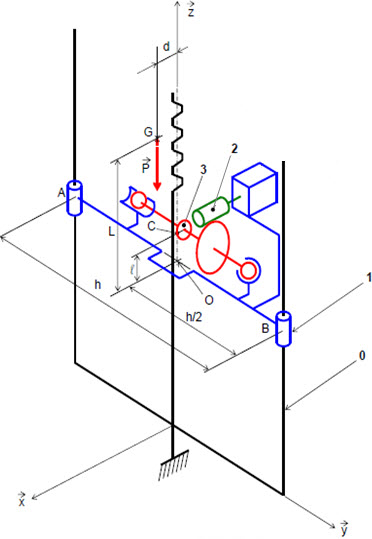
\includegraphics[width=\linewidth,height=.72\textheight,keepaspectratio]{images/image46.jpg}\textbf{Exemple~}:
Borne rétractable

Une borne rétractable est actionnée par un moteur associé à un réducteur
de réduction 60 et un dispositif pignon crémaillère qui permet de
transformer le mouvement de rotation en un mouvement de translation
rectiligne de la borne.


\includegraphics[width=\linewidth,height=.72\textheight,keepaspectratio]{images/image47.png}

\begin{enumerate}
\def\labelenumi{\arabic{enumi}.}
\item
  Déterminer la relation entre la vitesse angulaire de rotation du
  moteur et la vitesse de translation de la borne
  \(k = \frac{v_{1/0}}{\omega_{2/0}}\).
\end{enumerate}
\end{minipage} \\




\end{tabular}\end{center}

\subsubsection{Transmetteur cylindre roulant sans glisser sur un
plan}\label{transmetteur-cylindre-roulant-sans-glisser-sur-un-plan}

Tout \textbf{cylindre roulant sans glisser} sur un plan se comporte
\textbf{cinématiquement comme} un \textbf{transmetteur
pignon-crémaillère~:}
\(\left| \frac{\mathbf{v}_{\mathbf{s}}}{\mathbf{\omega}_{\mathbf{e}}} \right|\mathbf{= R}\)


\includegraphics[width=\linewidth,height=.72\textheight,keepaspectratio]{images/image48.png}

\subsubsection{\texorpdfstring{Transmetteur pignons-chaîne ou
poulies-courroie
}{Transmetteur pignons-chaîne ou poulies-courroie }}\label{transmetteur-pignons-chauxeene-ou-poulies-courroie}

Les dispositifs \textbf{poulies-courroie} ou \textbf{pignons-chaîne}
peuvent être également utilisés comme transformateur de mouvement.


\includegraphics[width=\linewidth,height=.72\textheight,keepaspectratio]{images/image49.png}

Les \textbf{deux poulies} ou les \textbf{deux pignons} ont \textbf{même
diamètre}.

Les \textbf{deux poulies} (ou \textbf{pignons}) sont guidées en
\textbf{rotation} par rapport au \textbf{bâti} et un brin de la
\textbf{courroie} (ou \textbf{chaîne}) en \textbf{translation} par
rapport au \textbf{bâti}. Ce transmetteur réalise une
\textbf{transformation de puissance} (rotation translation) \textbf{de
façon réversible}.

Utilisé comme transformateur de mouvement, un dispositif
\textbf{poulies-courroie} ou \textbf{pignons-chaîne} se comporte
\textbf{cinématiquement comme} un \textbf{transmetteur
pignon-crémaillère} :

Ils sont particulièrement avantageux lorsqu'il s'agit de relier de
grands entraxes. Ils sont alors moins coûteux que les transmissions par
engrenages. Ils sont utilisés dans tous secteurs de la construction
mécanique (machines-outils, convoyeurs, engins de travaux publics,
moteurs ...).

\textbf{NB~: Attention les roues ou poulies tournent dans le même sens
(contrairement aux engrenages).}

\subsubsection{Transmetteur vis-écrou}\label{transmetteur-vis-uxe9crou}


\includegraphics[width=\linewidth,height=.72\textheight,keepaspectratio]{images/image50.png}

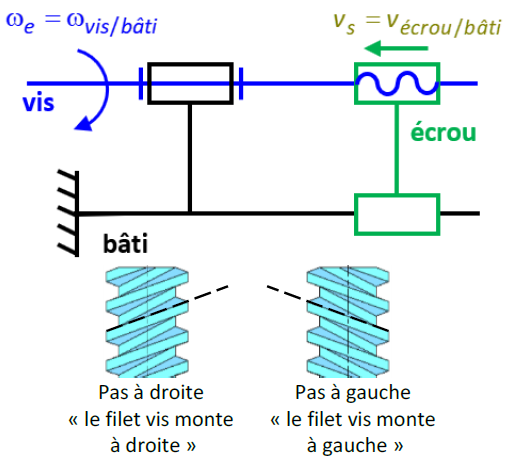
\includegraphics[width=\linewidth,height=.72\textheight,keepaspectratio]{images/image51.png}La
\textbf{vis} est guidée en \textbf{rotation} par rapport au
\textbf{bâti} et l'\textbf{écrou} en \textbf{translation} par rapport au
\textbf{bâti}. Ce transmetteur réalise une \textbf{transformation de
puissance} (rotation-translation) \textbf{de façon non-réversible} en
général.

Le modèle cinématique d'un dispositif vis-écrou est donné ci-contre. Sur
ce schéma les sens de rotation de la vis et de translation de l'écrou
correspondent au cas d'une vis avec pas à droite.

On peut remarquer le symbole d'une liaison hélicoïdale entre la vis et
l'écrou. Cette liaison modélise la possibilité d'un mouvement combiné de
rotation et translation suivant le même axe/direction.


\includegraphics[width=\linewidth,height=.72\textheight,keepaspectratio]{images/image52.png}

\begin{center}\begin{tabular}[]{@{}
  >{\raggedright\arraybackslash}p{0.1227\linewidth}
  >{\raggedright\arraybackslash}p{0.8773\linewidth}@{}}

\begin{minipage}[b]{\linewidth}\raggedright
\begin{quote}

\includegraphics[width=\linewidth,height=.72\textheight,keepaspectratio]{images/image30.png}
\end{quote}
\end{minipage} & \begin{minipage}[b]{\linewidth}\raggedright
\textbf{Exemple~}: Pilote automatique de bateau

Un pilote automatique électrique de bateau dont l'éclaté est donné
ci-dessous est étudié.


\includegraphics[width=\linewidth,height=.72\textheight,keepaspectratio]{images/image53.png}

\begin{enumerate}
\def\labelenumi{\arabic{enumi}.}
\item
  Donner la relation entre la vitesse de translation de la tige
  \textbf{4} du pilote et la vitesse de rotation de la MCC \textbf{15}
  sachant que le pas de la vis est de 4 mm,
  \(k = \frac{v_{4/0}}{\omega_{15/0}}\).
\end{enumerate}
\end{minipage} \\




\end{tabular}\end{center}

\begin{center}\begin{tabular}[]{@{}
  >{\raggedright\arraybackslash}p{0.1227\linewidth}
  >{\raggedright\arraybackslash}p{0.8773\linewidth}@{}}

\begin{minipage}[b]{\linewidth}\raggedright
\begin{quote}

\includegraphics[width=\linewidth,height=.72\textheight,keepaspectratio]{images/image30.png}
\end{quote}
\end{minipage} & \begin{minipage}[b]{\linewidth}\raggedright
\textbf{Exemple~}:


\includegraphics[width=\linewidth,height=.72\textheight,keepaspectratio]{images/image54.png}

\begin{enumerate}
\def\labelenumi{\arabic{enumi}.}
\item
  Donner le rapport de transmission,
  \(k = \frac{\omega_{8/0}}{\omega_{1/0}}\).
\end{enumerate}
\end{minipage} \\




\end{tabular}\end{center}

\begin{center}\begin{tabular}[]{@{}
  >{\raggedright\arraybackslash}p{0.1227\linewidth}
  >{\raggedright\arraybackslash}p{0.8773\linewidth}@{}}

\begin{minipage}[b]{\linewidth}\raggedright
\begin{quote}

\includegraphics[width=\linewidth,height=.72\textheight,keepaspectratio]{images/image30.png}
\end{quote}
\end{minipage} & \begin{minipage}[b]{\linewidth}\raggedright
\textbf{Objectif d'appareil photo~}:


\includegraphics[width=\linewidth,height=.72\textheight,keepaspectratio]{images/image8.png}

L'objectif photographique est équipé de deux capteurs permettant de
mesurer le déplacement de la lentille :

\begin{itemize}
\item
  un codeur absolu linéaire 4 bits, situé au niveau de la lentille
  mobile, permettant de connaitre la position de la lentille mobile
  selon la direction \(\overrightarrow{z_{0}}\) de la figure 4 ;
\end{itemize}


\includegraphics[width=\linewidth,height=.72\textheight,keepaspectratio]{images/image55.png}

\begin{itemize}
\item
  un codeur incrémental (monovoie, 30 impulsions par tour) relié à la
  MCC (Machine à Courant Continu) par un dispositif poulies-courroie .
\end{itemize}


\includegraphics[width=\linewidth,height=.72\textheight,keepaspectratio]{images/image56.png}

\begin{enumerate}
\def\labelenumi{\arabic{enumi}.}
\item
  Déterminer la relation entre le déplacement de la lentille mobile
  \(d_{l}\) et la position angulaire du codeur incrémental
  \(\theta_{rc}\). En déduire la résolution possible pour la course
  totale de la lentille, si elle est déterminée en\\
  comptant les impulsions du codeur incrémental sur les fronts montants.
\end{enumerate}\strut
\end{minipage} \\




& \\
\end{tabular}\end{center}

\subsubsection{\texorpdfstring{Transmetteur à train d'engrenages
épicycloïdal
}{Transmetteur à train d'engrenages épicycloïdal }}\label{transmetteur-uxe0-train-dengrenages-uxe9picyclouxefdal}

Pour obtenir un très grand rapport de transmission avec un train
d'engrenages simple, il faut utiliser plusieurs étages, ce qui est lourd
et encombrant. Les \textbf{trains d'engrenages épicycloïdaux} permettent
d'obtenir de grand rapport de réduction dans un encombrement faible.

\textbf{Constituants : Satellite, porte-satellite et planétaires}


\includegraphics[width=\linewidth,height=.72\textheight,keepaspectratio]{images/image57.png}

\begin{center}\begin{tabular}[]{@{}
  >{\raggedright\arraybackslash}p{0.2147\linewidth}
  >{\raggedright\arraybackslash}p{0.7853\linewidth}@{}}




\multicolumn{2}{@{}>{\raggedright\arraybackslash}p{(\columnwidth - 2\tabcolsep) * \real{1.0000} + 2\tabcolsep}@{}}{%
Les constituants d'un train d'engrenage épicycloïdal, à repérer dans cet
ordre, sont :} \\
\textbf{porte-satellite} & Pièce en rotation d'axe fixe par rapport au
bâti, sur laquelle sont montés des roues dentées : le(s)
satellite(s). \\
\textbf{satellite} & Roue dentée en rotation d'axe fixe par rapport au
porte-satellite ; \textbf{son axe de rotation n'est pas fixe par rapport
au bâti.} \\
\textbf{planétaires} & Roue dentée (pignon ou couronne) d'axe fixe par
rapport au bâti, qui engrène avec le(s) satellite(s). \\
\end{tabular}\end{center}

L'un des deux planétaires ou le porte-satellite peuvent être les pièces
d'entrée ou de sortie du transmetteur.

L'utilisation de plusieurs satellites ne modifie pas le comportement
cinématique du train épicycloïdal mais permet de mieux répartir les
efforts. C'est pour cette raison qu'un seul satellite apparait en
général sur les schémas cinématique.

\begin{center}\begin{tabular}[]{@{}
  >{\raggedright\arraybackslash}p{0.1227\linewidth}
  >{\raggedright\arraybackslash}p{0.8773\linewidth}@{}}

\begin{minipage}[b]{\linewidth}\raggedright
\begin{quote}

\includegraphics[width=\linewidth,height=.72\textheight,keepaspectratio]{images/image30.png}
\end{quote}
\end{minipage} & \begin{minipage}[b]{\linewidth}\raggedright

\includegraphics[width=\linewidth,height=.72\textheight,keepaspectratio]{images/image57.png}

Identifier les différentes pièces~:

Pla A (Planétaire A)~:

Pla B (Planétaire B)~:

PS (Porte-Satellite)~:

S (Satellite(s))
\end{minipage} \\




\end{tabular}\end{center}

\textbf{Rapport de transmission}

Si on observe le mouvement depuis le porte-satellite, on retrouve une
situation où tous les axes sont fixes (par rapport au porte-satellite),
comme dans le cas des trains d'engrenages simples vus plus tôt.

Pour déterminer la loi d'entrée-sortie d'un train épicycloïdal,
\textbf{on utilise la formule pour les trains simples, non-pas vue du
bâti mais du porte-satellite, en prenant comme entrée et sortie les
planétaires} :

Pour calculer la raison de base du train épicycloïdal, il suffit
d'imaginer que le porte-satellite est bloqué par rapport au bâti. Cela
transforme le train épicycloïdal en train simple.

Après avoir identifié les planétaires le(s) satellite(s) et le
porte-satellite grâce aux aides de repérage précédentes, on applique
directement une formule que l'on trouve dans la littérature, la formule
de Willis

\(\omega_{Pla.A/0} - \lambda.\omega_{Pla.B/0} + (\lambda - 1).\omega_{PS/0} = 0\)
avec
\(\lambda = \left. \ \frac{\omega_{Pla.A/0}}{\omega_{Pla.B/0}} \right|_{\omega_{PS/0} = 0}\)
(1\textsuperscript{ère} forme~: la plus pratique) ou
\(\frac{\omega_{Pla.A/0} - \omega_{PS/0}}{\omega_{Pla.B/0} - \omega_{PS/0}} = \lambda\)
avec
\(\lambda = \left. \ \frac{\omega_{Pla.A/0}}{\omega_{Pla.B/0}} \right|_{\omega_{PS/0} = 0}\)
(2\textsuperscript{ème} forme)

Où le paramètre

\includegraphics{images/image58.png}
\textbf{appelé raison de base} du train est une constante et correspond
au rapport de transmission du train d'engrenage simple obtenu en
immobilisant le porte satellite.

Remarque pour mieux retenir~: la somme des coefficients de la
1\textsuperscript{ère} forme est nulle~:

\includegraphics{images/image59.png}

'\,'

\textbf{2\textsuperscript{ème} méthode~:} on se ramène à un réducteur à
axes fixes en prenant le porte-satellite \ul{3} comme solide de
référence et en libérant en rotation \ul{0} par rapport à \ul{3} et on
déterminer la raison comme précédemment. On obtient ainsi~: :
\(\lambda = \frac{\text{\ensuremath{\omega}}_{\text{1/4}}}{\text{\ensuremath{\omega}}_{\text{3/4}}}\text{=-}\frac{\text{Z}_{\text{2}}\text{Z}_{\text{3}}}{\text{Z}_{\text{1}}\text{Z}_{\text{2}}}\text{ }\text{-}\frac{\text{Z}_{\text{3}}}{\text{Z}_{1}}\)

Puis on applique le théorème de composition des vitesses~:
\(\text{\ensuremath{\omega}}_{\text{1/3}} = \text{\ensuremath{\omega}}_{\text{1/0}} - \text{\ensuremath{\omega}}_{\text{3/0}}\)
\ldots{} pour faire apparaître le bâti.

\textbf{3\textsuperscript{ème} méthode~:} on utilise la propriété de
roulement sans glissement des cercles primitifs

\(\overrightarrow{V_{A \in 2/4}} = \overrightarrow{0}\) et
\(\overrightarrow{V_{B \in 2/3}} = \overrightarrow{0}\). De ces deux
relations on déduit deux équations qui combinées donnent la formule de
Willis.


\includegraphics[width=\linewidth,height=.72\textheight,keepaspectratio]{images/image60.png}

\textbf{Configuration}

Un train épicycloïdal a 3 entrées/sorties possibles :
\(\omega_{Pla.A/0}\), \(\omega_{Pla.B/0}\) et \(\omega_{PS/0}\).
L'utilisation d'un train épicycloïdal nécessite alors d'imposer la
vitesse angulaire par rapport au bâti de deux des trois entrées
possibles. Dans la pratique, on bloque souvent l'une d'entre-elles et
les deux autres sont l'entrée et la sortie.

\begin{center}\begin{tabular}[]{@{}
  >{\raggedright\arraybackslash}p{0.1227\linewidth}
  >{\raggedright\arraybackslash}p{0.8773\linewidth}@{}}

\begin{minipage}[b]{\linewidth}\raggedright
\begin{quote}

\includegraphics[width=\linewidth,height=.72\textheight,keepaspectratio]{images/image30.png}
\end{quote}
\end{minipage} & \begin{minipage}[b]{\linewidth}\raggedright

\includegraphics[width=\linewidth,height=.72\textheight,keepaspectratio]{images/image57.png}

\begin{enumerate}
\def\labelenumi{\arabic{enumi}.}
\item
  Déterminer le rapport de réduction
  \(k = \frac{\omega_{3/0}}{\omega_{1/0}}\) si on considère le solide 4
  relié au bâti.
\item
  Déterminer le rapport de réduction
  \(k = \frac{\omega_{4/0}}{\omega_{1/0}}\) si on considère le solide 3
  relié au bâti.
\item
  Déterminer le rapport de réduction
  \(k = \frac{\omega_{3/0}}{\omega_{4/0}}\) si on considère le solide 1
  relié au bâti.
\end{enumerate}
\end{minipage} \\




\begin{minipage}[t]{\linewidth}\raggedright
\begin{quote}

\includegraphics[width=\linewidth,height=.72\textheight,keepaspectratio]{images/image30.png}
\end{quote}
\end{minipage} &

\includegraphics[width=\linewidth,height=.72\textheight,keepaspectratio]{images/image61.png} \\
& Dans cet exemple, on parle de satellite double. \\
\end{tabular}\end{center}

\textbf{Les différents types de trains épicycloïdaux}

Pour obtenir un rapport de vitesse (que ce soit par la méthode 1, 2 ou
3), il faut qu\textquotesingle un arbre (\ul{1}, \ul{3} ou \ul{4}) soit
moteur, un arbre soit récepteur et un arbre soit bloqué lié au bâti.

Dans le cas des trains parallèles, les deux planétaires engrenant avec
les satellites peuvent être situés autour (cas des planétaires
extérieurs), ou au centre (cas des planétaires intérieurs). Il en
résulte 4 configurations.

\begin{center}\begin{tabular}[]{@{}
  >{\raggedright\arraybackslash}p{0.5000\linewidth}
  >{\raggedright\arraybackslash}p{0.5000\linewidth}@{}}

\begin{minipage}[b]{\linewidth}\raggedright

\includegraphics[width=\linewidth,height=.72\textheight,keepaspectratio]{images/image62.png}

satellite à simple denture, un planétaire intérieur et un extérieur
\end{minipage} & \begin{minipage}[b]{\linewidth}\raggedright

\includegraphics[width=\linewidth,height=.72\textheight,keepaspectratio]{images/image63.png}

satellite à double denture un planétaire intérieur et un extérieur
\end{minipage} \\





\includegraphics[width=\linewidth,height=.72\textheight,keepaspectratio]{images/image64.png}

satellite à double denture et 2 planétaires intérieurs &

\includegraphics[width=\linewidth,height=.72\textheight,keepaspectratio]{images/image65.png}

satellite à double denture et 2 planétaires extérieurs \\
\multicolumn{2}{@{}>{\raggedright\arraybackslash}p{(\columnwidth - 2\tabcolsep) * \real{1.0000} + 2\tabcolsep}@{}}{%

\includegraphics[width=\linewidth,height=.72\textheight,keepaspectratio]{images/image66.png}

Schéma d\textquotesingle un différentiel~: le porte satellite (en bleu)
constitue l\textquotesingle entrée du dispositif, et les deux
planétaires (rouge et jaune) les sorties dont la vitesse de rotation
peut être différente.} \\
\end{tabular}\end{center}

\subsection{QUELQUES DISPOSITIFS
SUPPLEMENTAIRES}\label{quelques-dispositifs-supplementaires}

\begin{center}\begin{tabular}[]{@{}
  >{\raggedright\arraybackslash}p{0.0556\linewidth}
  >{\raggedright\arraybackslash}p{0.4586\linewidth}
  >{\raggedright\arraybackslash}p{0.4858\linewidth}@{}}

\begin{minipage}[b]{\linewidth}\raggedright
\textbf{Bielle-manivelle}
\end{minipage} & \begin{minipage}[b]{\linewidth}\raggedright

\includegraphics[width=\linewidth,height=.72\textheight,keepaspectratio]{images/image67.png}

Pièce 1~: manivelle (ou maneton ou vilebrequin)

Pièce 2~: bielle

Pièce 3~: piston (ou coulisseau)
\end{minipage} & \begin{minipage}[b]{\linewidth}\raggedright
\begin{quote}
\textbf{Transformation~:}

Rotation continue en translation alternative (et réciproquement
parfois).

\textbf{Réversibilité~:} parfois.

\textbf{Utilisation~:}

Moteurs thermiques, compresseurs, certaines pompes et moteurs
hydrauliques, marteau perforateur\ldots{}

NB~: Dans un moteur thermique ou une pompe, le bâti au niveau du piston
s'appelle chemise ou cylindre.

\textbf{Caractéristiques~:}


\includegraphics{images/image68.png}

\includegraphics{images/image69.png}

Très souvent~: L\textgreater\textgreater e (L\textgreater5.e suffit en
général pour pouvoir faire cette hypothèse).
\end{quote}
\end{minipage} \\




\textbf{Pignon-crémaillère} &

\includegraphics[width=\linewidth,height=.72\textheight,keepaspectratio]{images/image70.png}
& \begin{minipage}[t]{\linewidth}\raggedright
\begin{quote}
\textbf{Transformation~:}

Rotation continue en translation continue (et réciproquement).

\textbf{Réversibilité~:} toujours.

\textbf{Utilisation~:}

Porte de TGV, porte de garage, direction de voiture, bras
manipulateur\ldots{}

\textbf{Caractéristiques~:}

Diamètre du pignon.
\end{quote}
\end{minipage} \\
\end{tabular}\end{center}

\begin{center}\begin{tabular}[]{@{}
  >{\raggedright\arraybackslash}p{0.0541\linewidth}
  >{\raggedright\arraybackslash}p{0.4462\linewidth}
  >{\raggedright\arraybackslash}p{0.4998\linewidth}@{}}

\begin{minipage}[b]{\linewidth}\raggedright
\textbf{Vis-écrou}
\end{minipage} & \begin{minipage}[b]{\linewidth}\raggedright

\includegraphics[width=\linewidth,height=.72\textheight,keepaspectratio]{images/image71.jpeg}

\begin{quote}
Pièce 1~: vis
\end{quote}

Pièce 2~: coulisseau (ou écrou)
\end{minipage} & \begin{minipage}[b]{\linewidth}\raggedright
\begin{quote}
\textbf{Transformation~:}

Rotation continue en translation continue.

\textbf{Réversibilité~:} parfois. Elle dépend des matériaux en contact
et de l'angle de l'hélice.

\textbf{Utilisation~:}

Vérins électriques, chariots de machine-outil, pilote automatique,
élévateur...

\textbf{Caractéristiques~:}

Pas de la vis~: p (mm) à droite
\end{quote}
\end{minipage} \\




\begin{minipage}[t]{\linewidth}\raggedright
\textbf{\hfill\break
}\textbf{Croix de Malte}\strut
\end{minipage} &

\includegraphics[width=\linewidth,height=.72\textheight,keepaspectratio]{images/image72.png}
& \begin{minipage}[t]{\linewidth}\raggedright
\begin{quote}
\textbf{Transformation~:}

Rotation continue en rotation intermittente.

\textbf{Réversibilité~:} jamais.

\textbf{Utilisation~:}

Plateau tournant de machine de transfert, indexage\ldots{}

\textbf{Caractéristiques~:}

Angle entre les différentes rainures, et rayon de l'ergot.
\end{quote}
\end{minipage} \\
\textbf{Excentrique} &

\includegraphics[width=\linewidth,height=.72\textheight,keepaspectratio]{images/image73.jpeg}

Pièce 1~: excentrique

Pièce 2~: piston (ou coulisseau) &
\begin{minipage}[t]{\linewidth}\raggedright
\begin{quote}
\textbf{Transformation~:}

Rotation continue en translation alternative.

\textbf{Réversibilité~:} jamais.

\textbf{Utilisation~:}

Pompes hydrauliques, taille haie, certains mécanismes d'ablocage
(blocage d'une pièce sur une table).

\textbf{Caractéristiques~:}


\includegraphics{images/image74.png}

\includegraphics{images/image68.png}
\end{quote}
\end{minipage} \\
\end{tabular}\end{center}

\begin{center}\begin{tabular}[]{@{}
  >{\raggedright\arraybackslash}p{0.0541\linewidth}
  >{\raggedright\arraybackslash}p{0.4462\linewidth}
  >{\raggedright\arraybackslash}p{0.4998\linewidth}@{}}

\begin{minipage}[b]{\linewidth}\raggedright
\textbf{Came axiale}
\end{minipage} & \begin{minipage}[b]{\linewidth}\raggedright

\includegraphics[width=\linewidth,height=.72\textheight,keepaspectratio]{images/image75.jpeg}

Pièce 1~: came (ici un plateau incliné)

La came peut être un cylindre sur lequel est usinée une rainure de forme
quelconque.
\end{minipage} & \begin{minipage}[b]{\linewidth}\raggedright
\begin{quote}
\textbf{Transformation~:}

Rotation continue en translation alternative.

\textbf{Réversibilité~:} jamais.

\textbf{Utilisation~:} Pompes hydrauliques.

\textbf{Caractéristiques~:}


\includegraphics{images/image76.png}

\includegraphics{images/image77.png}

Le plan

\includegraphics{images/image78.png}
définit le plateau.
\end{quote}
\end{minipage} \\




\end{tabular}\end{center}

\subsection{Sources}\label{sources}

Ce cours a été élaboré à l'aide de nombreuses ressources~provenant de
documents publics d'industriels, des activités pédagogiques de collègues
de l'UPSTI.

\subsection{Exercices du chapitre}\label{exercices-du-chapitre}


\includegraphics[width=\linewidth,height=.72\textheight,keepaspectratio]{images/image79.png}

\textbf{TRAINS EPICYCLOIDAUX}


\includegraphics[width=\linewidth,height=.72\textheight,keepaspectratio]{images/image800.png}
Niveau 2

\begin{enumerate}
\item
  Déterminer le rapport de réduction du réducteur épicycloïdal ATV
  suivant~:
\end{enumerate}


\includegraphics[width=\linewidth,height=.72\textheight,keepaspectratio]{images/image81.png}\(\mathbf{z}_{\mathbf{1}}\mathbf{= 166;}\mathbf{z}_{\mathbf{2}}\mathbf{= 160;}\mathbf{z}_{\mathbf{2}\mathbf{'}}\mathbf{= 164;}\mathbf{z}_{\mathbf{3}}\mathbf{= 170;}\)

\textbf{Déterminer} le rapport de réduction du réducteur épicycloïdal du
sécateur Pellenc.


\includegraphics[width=\linewidth,height=.72\textheight,keepaspectratio]{images/image82.png}\(\mathbf{z}_{\mathbf{1}}\mathbf{= 19;}\mathbf{z}_{\mathbf{2}}\mathbf{= 19;}\mathbf{z}_{\mathbf{3}}\mathbf{= 57;}\)

3

\textbf{TRAIN D'ENGRENAGE SIMPLE}


\includegraphics[width=\linewidth,height=.72\textheight,keepaspectratio]{images/image800.png}
Niveau 1

Un train d'engrenage, dans lequel toutes les roues dentées sont en
mouvement de rotation d'axes parallèles par rapport au bâti, est
représenté sur la figure ci-dessous~:


\includegraphics[width=\linewidth,height=.72\textheight,keepaspectratio]{images/image83.png}

Z\textsubscript{1} = 65 dents

Z\textsubscript{2} = 32 dents

Z\textsubscript{3} = 24 dents~- Z\textsubscript{3'}= 48 dents

Z\textsubscript{4} = 38 dents~- Z\textsubscript{4'} = 82 dents

Z\textsubscript{5} = 26 dents - Z\textsubscript{5'} = 54 dents

Z\textsubscript{6} = 42 dents

Z\textsubscript{7} = 30 dents

\textbf{Q1.} Indiquer, à l'aide de flèches, le sens de rotation de
chacune des roues dentées.

\textbf{Q2}. Lister les roues dentées considérées comme menantes et les
roues dentées considérées comme menées.

\textbf{Q3.} Donner l'expression du rapport de transmission
\(k = \frac{\omega_{e/0}}{\omega_{s/0}}\) du train d'engrenages.

\textbf{Q4}. Faire l'application numérique. En déduire s'il s'agit d'un
réducteur ou d'un multiplicateur de vitesse


\includegraphics[width=\linewidth,height=.72\textheight,keepaspectratio]{images/image84.png}\textbf{MONTE-CHARGE}


\includegraphics[width=\linewidth,height=.72\textheight,keepaspectratio]{images/image800.png}
Niveau 2

Le monte-charge représenté ci-contre utilise un moteur (1500 tr/min)
associé à un réducteur du fabricant DEMAG pour enrouler un câble sur un
tambour et faire ainsi monter une charge.


\includegraphics[width=\linewidth,height=.72\textheight,keepaspectratio]{images/image85.png}La
représentation technique 2D du réducteur utilisé, est donnée ci-dessous.
Caractéristiques des roues dentées~:

\begin{center}\begin{tabular}[]{@{}
  >{\raggedright\arraybackslash}p{0.3333\linewidth}
  >{\raggedright\arraybackslash}p{0.3333\linewidth}
  >{\raggedright\arraybackslash}p{0.3333\linewidth}@{}}

\begin{minipage}[b]{\linewidth}\raggedright
\textbf{Rep}
\end{minipage} & \begin{minipage}[b]{\linewidth}\raggedright
\textbf{m}
\end{minipage} & \begin{minipage}[b]{\linewidth}\raggedright
\textbf{Z}
\end{minipage} \\




6 & 1 & 16 \\
9a & 1 & 46 \\
9b & 1 & 19 \\
11a & 1 & 59 \\
11b & 1,25 & 17 \\
16 & 1,25 & 85 \\
\end{tabular}\end{center}

6

11

9

16

2

Pour obtenir un temps de montée minimal, tout en limitant la norme de
l'accélération pendant le démarrage qui pourrait être à l'origine de
dégâts sur la charge transportée, on impose le profil de vitesse
suivant.

\textbf{Q1.} Identifier, en les coloriant, les différentes CEC du
réducteur.

\textbf{Q2.} Dessiner le schéma cinématique du réducteur dans le plan
correspondant à la vue en coupe C-C.

\textbf{Q3.} Donner l'expression du rapport de réduction
\(i = \frac{\omega_{s/2}}{\omega_{e/2}}\) du réducteur.

\textbf{Q4}. Faire l'application numérique.


\includegraphics[width=\linewidth,height=.72\textheight,keepaspectratio]{images/image90.jpeg}On
désire obtenir, en utilisant un réducteur roue et vis sans fin dont la
vis possède 4 filets, le même rapport de réduction que le réducteur
étudié dans l'exercice du monte-charge.

\textbf{Q5}. Déterminer le nombre de dents de la roue dentée.

\textbf{PORTAIL AUTOMATISE}


\includegraphics[width=\linewidth,height=.72\textheight,keepaspectratio]{images/image800.png}
Niveau 2


\includegraphics[width=\linewidth,height=.72\textheight,keepaspectratio]{images/image91.png}On
s'intéresse à la chaîne d\textquotesingle énergie d\textquotesingle un
portail automatisé et plus particulièrement au réducteur utilisé. La
mise en mouvement du vantail se fait à l'aide d\textquotesingle un
moteur électrique qui transmet l'énergie mécanique de rotation, par
l'intermédiaire d'un réducteur, au bras de commande lié au vantail (voir
figure sur la page suivante).

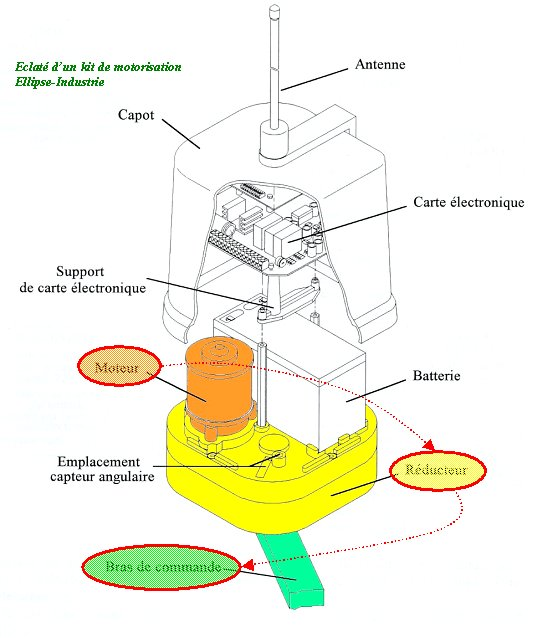
\includegraphics[width=\linewidth,height=.72\textheight,keepaspectratio]{images/image92.jpeg}
\includegraphics[width=\linewidth,height=.72\textheight,keepaspectratio]{images/image93.png}

Le moteur \textbf{21} (3000 tr~/min) entraîne le pignon moteur
\textbf{19} qui, par les différents trains d'engrenages du réducteur
\textbf{19-5} (m=0,75), \textbf{3-22} (m=0,75), \textbf{23-17} (m=1) et
\textbf{16-11 (}m=1,5), transmet le mouvement à l'arbre \textbf{9} (lié
au bras de commande) qui pivote de 90° pour permettre l'ouverture ou la
fermeture complète du ventail.

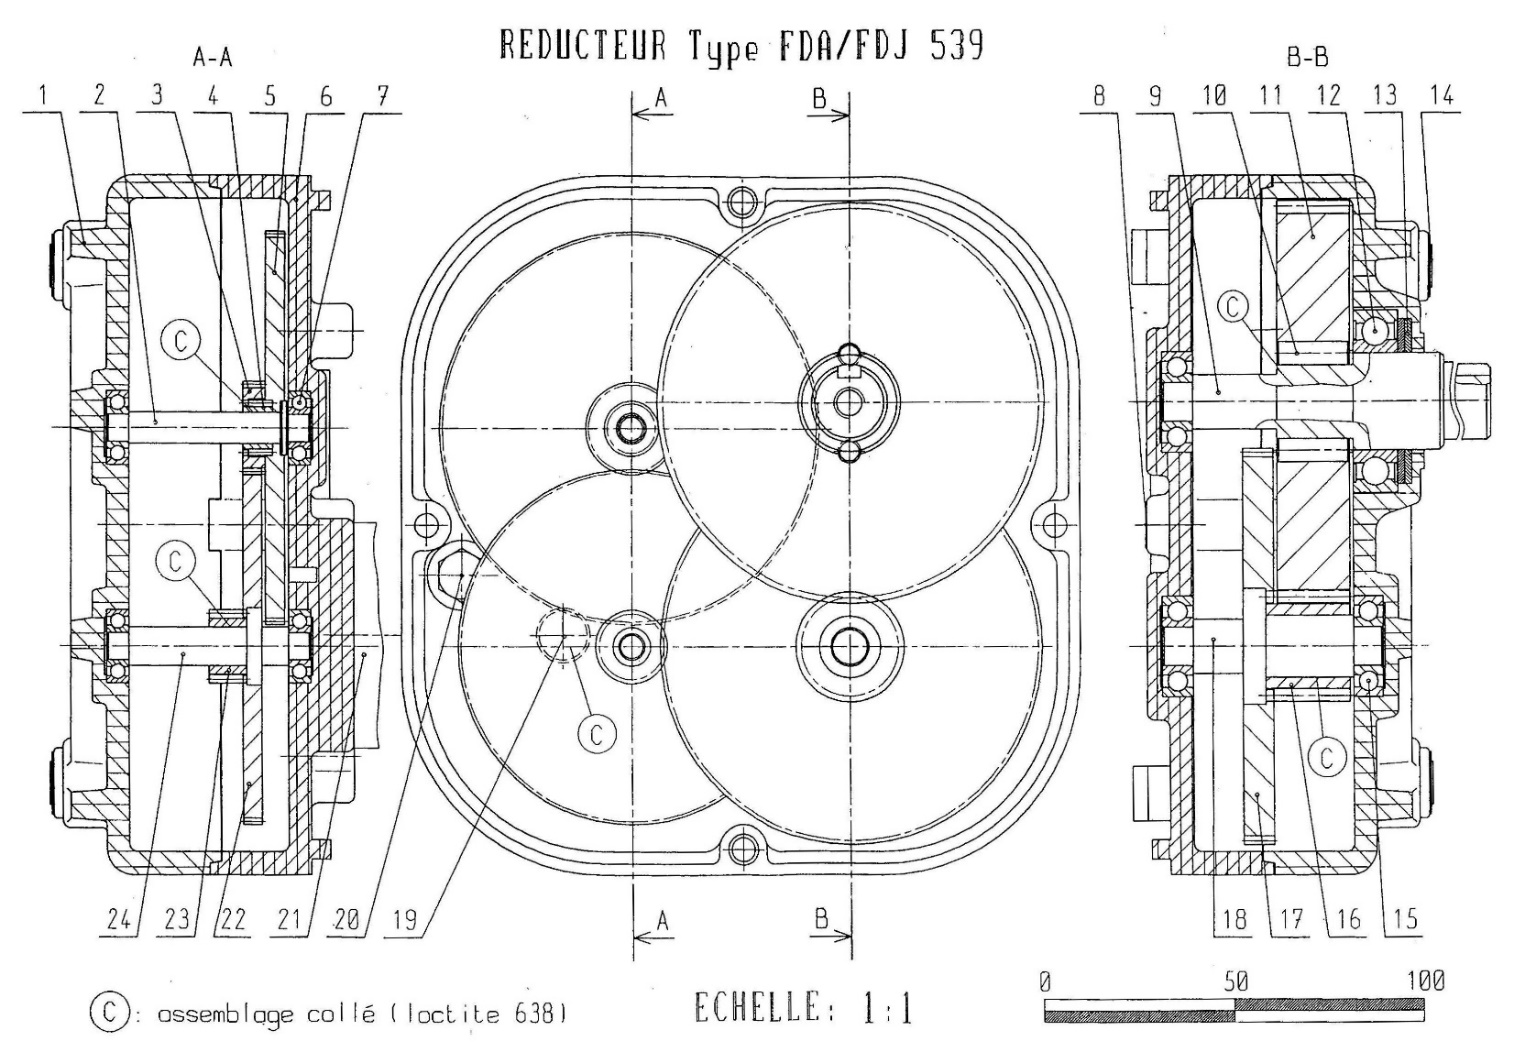
\includegraphics[width=\linewidth,height=.72\textheight,keepaspectratio]{images/image94.jpeg}Une
représentation technique 2D du réducteur est donnée ci-dessous.

1~: 2


\includegraphics[width=\linewidth,height=.72\textheight,keepaspectratio]{images/image95.png}

\textbf{\ul{Objectif~:}} Vérifier le critère de la fonction FP1.

\textbf{Q1.} Donner l'expression du rapport de réduction
\(r = \frac{\omega_{s/1}}{\omega_{e/1}}\) en fonction des diamètres
primitifs

\includegraphics{images/image96.png}des
roues dentées.

\textbf{Q2}. Faire l'application numérique.

\textbf{Q3}. Conclure quant au respect du critère de la fonction FP1.

\textbf{ROUE D'ENGIN}


\includegraphics[width=\linewidth,height=.72\textheight,keepaspectratio]{images/image800.png}
Niveau 4

Un réducteur de vitesse est souvent intégré dans le moyeu de roue des
engins de travaux publics. L\textquotesingle utilisation de deux trains
épicycloïdaux permet d\textquotesingle obtenir une solution très
compacte.

La pièce \ul{7} est liée à l\textquotesingle engin et constitue le bâti
fixe. L\textquotesingle arbre d\textquotesingle entrée \ul{1} est
entraînée en rotation par un moteur hydraulique (non représenté). La
roue est fixée sur la pièce \ul{12}.

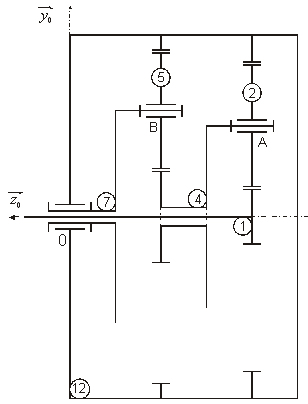
\includegraphics[width=\linewidth,height=.72\textheight,keepaspectratio]{images/image97.jpeg}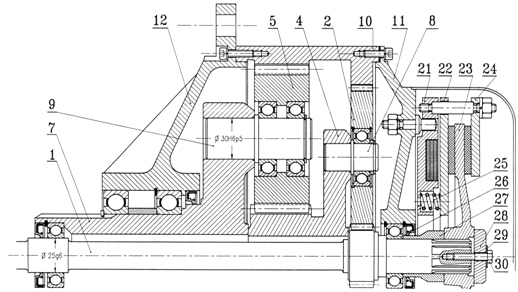
\includegraphics[width=\linewidth,height=.72\textheight,keepaspectratio]{images/image98.jpeg}

\emph{\textbf{\ul{Objectif~:}}} déterminer le rapport de réduction du
réducteur~: \(\frac{\omega_{12/7}}{\omega_{1/7}}\)

\textbf{\ul{Qu. 1}} Etudier le premier train et établir une relation
entre \(\omega_{1/7}\), \(\omega_{4/7}\) et \(\omega_{12/7}\).

\textbf{\ul{Qu. 2}} Etudier le second train et établir une relation
entre \(\omega_{4/7}\), et \(\omega_{12/7}\).

\textbf{\ul{Qu. 3}} A partir des réponses aux deux questions
précédentes, en déduire le rapport de réduction du réducteur
\(\frac{\omega_{12/7}}{\omega_{1/7}}\).

\emph{\textbf{\ul{Caractéristiques des engrenages~:}}}

\begin{itemize}
\item
  \emph{Train 1 :} pièces 1, 2, 4, 12
\end{itemize}

m = 2

Z\textsubscript{1} = 21 ; Z\textsubscript{2} = 51 ; Z\textsubscript{12a}
= 123

\begin{itemize}
\item
  \emph{Train 2 :} pièces 4, 5, 7, 12
\end{itemize}

m = 3

Z\textsubscript{4} = 23 ; Z\textsubscript{5} = 34 ; Z\textsubscript{12b}
= 91

\textbf{POULIE REDEX}


\includegraphics[width=\linewidth,height=.72\textheight,keepaspectratio]{images/image800.png}
Niveau 3


\includegraphics[width=\linewidth,height=.72\textheight,keepaspectratio]{images/image99.png}

Objectif~: Déterminer le rapport de réduction du réducteur
\(\frac{\omega_{31/0}}{\omega_{5/0}}\).

\textbf{ROBOT ERICC}


\includegraphics[width=\linewidth,height=.72\textheight,keepaspectratio]{images/image800.png}
Niveau 2

On s'intéresse au réducteur poulie-courroie crantée utilisé dans la
chaine d'énergie du mouvement de lacet du robot Ericc. La poulie motrice
\textbf{18}, liée à l'arbre de sortie du moto-réducteur, est en liaison
pivot par rapport au socle chaise \textbf{10}. La poulie réceptrice
\textbf{23} est fixe par rapport au bâti. Cela permet au socle chaise
\textbf{10}, en liaison pivot par rapport au bâti, de pivoter autour de
l'axe du lacet lors de la mise en marche du moto-réducteur.


\includegraphics[width=\linewidth,height=.72\textheight,keepaspectratio]{images/image100.png}

La représentation technique 2D du réducteur est donnée ci-dessous.

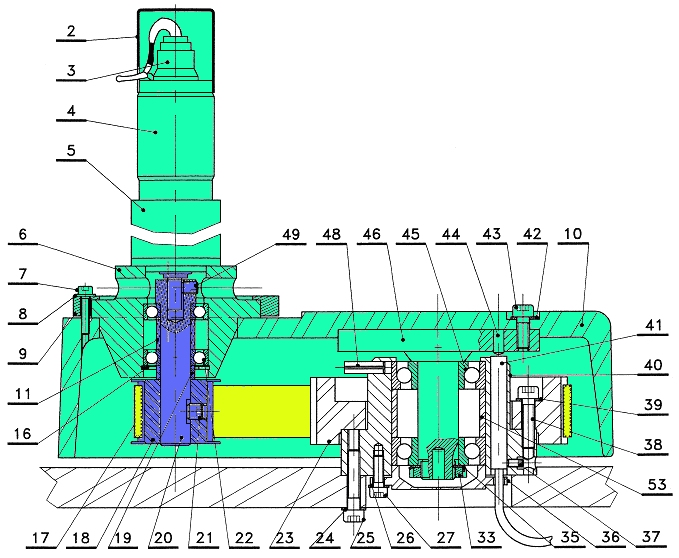
\includegraphics[width=\linewidth,height=.72\textheight,keepaspectratio]{images/image101.jpeg}

Le schéma cinématique du réducteur est donné ci-dessous.


\includegraphics[width=\linewidth,height=.72\textheight,keepaspectratio]{images/image102.png}

\textbf{Q1.} Donner l'expression du rapport de réduction
\(r = \frac{\omega_{23/10}}{\omega_{18/10}}\) en fonction des nombres de
dents des poulies.

\textbf{Q2}. En déduire la vitesse de rotation du robot autour de l'axe
vertical lorsque le moto-réducteur tourne à la vitesse maximale de 50
tr/min.

\textbf{\ul{\hfill\break
}}

\textbf{DESSILEUSE}


\includegraphics[width=\linewidth,height=.72\textheight,keepaspectratio]{images/image800.png}
Niveau 2

De nos jours les exploitations agricoles sont équipées de machines à
fonctions multiples ce qui permet à un seul exploitant de faire face à
de grosses charges de travail. La dessileuse, pailleuse, distributrice
ci-dessous en est un exemple. Cette machine a pour fonction de~:

\begin{itemize}
\item
  DESSILER~: prendre au silo, l'ensilage d'herbe et de maïs.
\item
  DISTRIBUER dans l'auge le produit.
\item
  PAILLER les aires d'exercice des animaux.
\end{itemize}

Nous allons étudier les systèmes de dessilage et de distribution. Ils
permettent à l'utilisateur par simple action sur des commandes
hydrauliques de charger l'ensilage dans la dessileuse puis de le
distribuer, grâce à une commande mécanique, aux animaux.

En effet, afin d'amplifier le couple d'effort transmis à la turbine de
distribution d'ensilage, il est prévu de réduire la fréquence de
rotation de l'arbre de sortie de la boite de vitesse.

Q1. Expliquer en quelques lignes la solution constructive retenue pour
réaliser la sélection petite vitesse.

Q2. Construire le schéma cinématique minimal du réducteur (en phase de
fonctionnement petite vitesse)

Q3. Expliquer en quelques lignes comment est réalisé le guidage en
rotation de l'arbre 7. On précisera notamment le type
d\textquotesingle éléments standards utilisés, et la façon dont les
arrêts axiaux sont réalisés.

Q4. Calculer le rapport de transmission
\(i = \frac{\omega_{sortie}}{\omega_{entrée}}\) du système étudié (en
phase de fonctionnement petite vitesse). Conclusion, comment peut-on
qualifier cette transmission~?

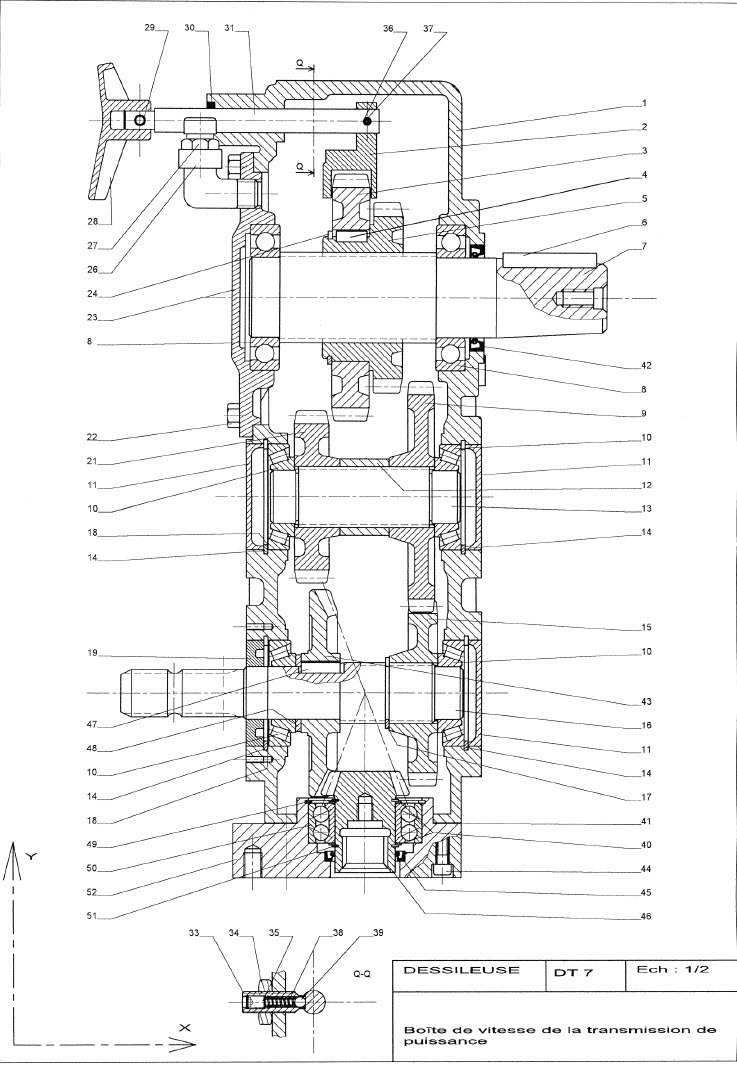
\includegraphics[width=\linewidth,height=.72\textheight,keepaspectratio]{images/image103.jpeg}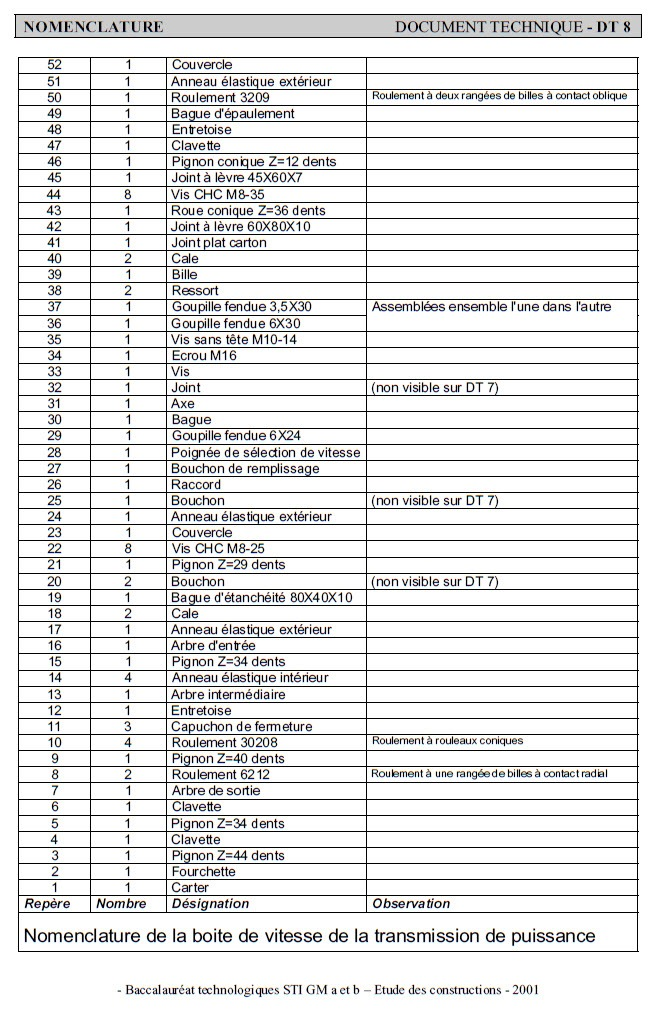
\includegraphics[width=\linewidth,height=.72\textheight,keepaspectratio]{images/image104.jpeg}

\textbf{COFFRE DE VOITURE}


\includegraphics[width=\linewidth,height=.72\textheight,keepaspectratio]{images/image800.png}
Niveau 2


\includegraphics[width=\linewidth,height=.72\textheight,keepaspectratio]{images/image105.png}Certaines
voitures sont dotées en série d'un système d'ouverture et de fermeture
du hayon de coffre électrique.

Ce système est constitué d'un moteur électrique de puissance nominale
150 W, dont la vitesse angulaire nominale est égale à 3300 tr/min.

La rotation du rotor de ce moteur est transmise au hayon par
l'intermédiaire d'un réducteur de vitesse, puis d'un transmetteur
\textbf{« 4 barres »} (CD-DB-BA-AC) dont une photo et un schéma
cinématique sont donnés ci-après.

L'ouverture du hayon est réalisée pour un angle de rotation de la
manivelle 4 de 68,4°. (\emph{Vidéos de mise en situation et du
fonctionnement sur le site internet).}

\begin{center}\begin{tabular}[]{@{}
  >{\raggedright\arraybackslash}p{0.3985\linewidth}
  >{\raggedright\arraybackslash}p{0.6015\linewidth}@{}}




Extrait du cahier des charges : Ex1 & le coffre motorisé doit s'ouvrir
sur une durée comprise \textbf{entre 3 et 5 secondes}. \\
\end{tabular}\end{center}


\includegraphics[width=\linewidth,height=.72\textheight,keepaspectratio]{images/image106.png}


\includegraphics[width=\linewidth,height=.72\textheight,keepaspectratio]{images/image107.png}

Une représentation 3D du réducteur de vitesse (+ la biellette 3) est
donnée ci-après.

\textbf{Le rotor 2 du moteur} est solidaire de la vis-sans-fin.


\includegraphics[width=\linewidth,height=.72\textheight,keepaspectratio]{images/image108.png}

\begin{enumerate}
\def\labelenumi{\arabic{enumi}.}
\item
  Déterminer l'expression du rapport de transmission
  \(i = \frac{\omega_{4/0}}{\omega_{2/0}}\). Faire l'application
  numérique.
\item
  En déduire la vitesse angulaire \(\omega_{4/0}\) en tr/min si le
  moteur tourne à sa vitesse nominale, puis le temps de fermeture T du
  coffre. Conclure sur le respect du cahier des charges.
\end{enumerate}
